\section{Intrusion detection fusion}
\label{sec:ids-fusion}
% \longidses ({\idses}) are systems that sense intrusions in computer networks and
% hosts.  
{\ids} fusion % \footnote{In the computer security community, this process is often called ``\ids
% correlation,'' but we prefer ``fusion'' as it more accurately describes the
% process, and doesn't collide with statistical terminology.
% Indeed, in some cases the term ``\ids correlation'' is not used to describe an
% automated process, but rather a human-executed process of investigating an
% \ids-generated alert~\cite[e.g.]{drew14:_what_role_secur_event_correl_intrus_detec}.} 
is the
problem of creating a
coherent overall picture of network status out of reports from multiple
{\idses} scattered around a computer network. % we wish to defend.  
An \ids fusion system must answer two questions:
\begin{compactenum}
\item How do the reports issued by the \idses correspond to events? Multiple
  reports, from the same \ids or from different \idses,  might
  actually refer to the same event. This is the problem of \emph{clustering}
  reports into events.
\item Which hypothesized events do we accept as actual?  This is the problem of
  \emph{assessing} the likelihood of event hypotheses.
\end{compactenum}
Goldman and Harp discuss the first of these two
questions~\shortcite{goldman:09Scyllarus}.  In this paper we will
focus on the second question, assuming a solution to the first.

Existing \idses are not designed to work together as part of a
suite of sensors.  Instead, each program generates a separate,
often voluminous, stream of reports; fusing them into a coherent 
overview is left
% TODO restore to QR15
%as an exercise for
 to
the user. 
Ideally, network administrators would have a suite of different \idses active,
since different \ids approaches
% TODO restore to QR15
% --- network (NIDS) vs.\
% host-based (HIDS), signature vs.\ anomaly-based --- 
bring different
strengths and weaknesses.
%%
%% Hm, can we just get rid of the details NIDS/HIDS and
%% signature/anomaly comparisons, and keep just the takeaway? I don't
%% believe we refer to them after this. 
%%
Briefly, more accurate \idses have significantly higher software
administration burdens, and there is an inevitable tradeoff between
false positives and false negatives.
This tradeoff applies for all of the different varieties of IDS,
for example NIDS or HIDS, signature-based, anomaly-detecting, various
hybrids.  We do not discuss the varieties of \idses here;
we are not concerned with the mechanics of clustering reports, but
rather with the subsequent assessment of hypothesized events.
%%
%%Some systems aim to overcome the limitations of existing \idses by assembling 
%%a suite of
%%sensors.  This can be a very efficient way to overcome the problem
%%of false positives, but relies crucially on finding sensors that fail
%%relatively independently.  
%%
%% 
%% NIDS systems are easy to deploy; from only one
%% or two locations, they can watch all relevant traffic.  Unfortunately, they also have
%% substantial problems with false positives and false negatives, because they
%% don't ``know'' the meaning of the traffic they see.  Often they must draw
%% conclusions based only on information in packet headers (although some
%% systems do attempt to reconstruct higher level protocols from packet data),
%% and more extensive reasoning about traffic either would slow down the
%% network, or must ignore some packets altogether.
%% A HIDS may take into account much more information about the state
%% of a defended system, but installing HIDS pervasively involves deploying and
%% configuring much more software.  Typically HIDS are installed on only the most
%% critical assets.
%% 
%% Signature-based systems attempt to match patterns of known bad behavior.  Such
%% \idses are plagued by false negatives, both because of novel attacks for which
%% there are no patterns to match, and because of known %knowledgeable attackers take
%% countermeasures against signature identification (e.g.\ encrypting malware, or
%% permuting its structure).  Anomaly detectors are prone to false
%% positives: anomalies are often benignly anomalous,
%% not maliciously so.  Detectors often believe there is an
%% anomaly when none exists because computer usage patterns are
%% notoriously difficult to learn: they are often non-stationary, they vary
%% substantially from location-to-location, etc.
%% \draft{Add citations of papers on the challenges of anomaly detection.}
 
The most substantial challenge in managing \idses is the information overload
that they can impose.
Much of this overload comes from the high false positive rate.  This rate is
partly due to
inaccurate sensors.
Another problem is the ``base rate fallacy''~\cite{Axelsson:1999:BFI:319709.319710}:
in intrusion detection, as in
other applications where very unlikely events must be detected, even a seemingly
accurate sensor may yield too many false positives.  Axelsson gives the example
of a 99\% accurate test detecting a disease that strikes only 1/10,000
patients.  
Although the sensor is accurate, 
the probability of having the disease given a positive test result is
only 1\%.
% %% This next bit seem redundant.
%, although the probability of the sensor labeling correctly is 99\%.

Users regularly ignore or disable their {\idses}, unable to absorb
massive streams of false alarms.
%% TODO Restore for QR'15
%``Users attending an 'ABCs of IDS' event at London's City University yesterday
%  said more the 80 per cent of the alerts they received were false, with one
%  citing 60 alerts he had received about non-existent problems that morning at
%  0300''
% ~\cite{Register}.
Recently, Target is reported to have ignored warnings about the
data breach that resulted in theft of millions of credit
card records~\cite{TargetIgnoredIDS}:
``They are bombarded with alerts. They get so many that they just don't respond
to everything''~\cite{finkle14:_target}.
Figure
\ref{fig:workloadReduction} gives a sense of the gravity of this
problem. It shows how our earlier system was able to winnow
the 
flow of reports in a small corporate network~\anoncite{goldman:09Scyllarus}.
% Data reduction must join building a comprehensive overview
% and overcoming false positives and negatives as goals of \ids fusion.
\begin{figure}[t]
    \ifthenelse{\boolean{blackAndWhite}}{%
      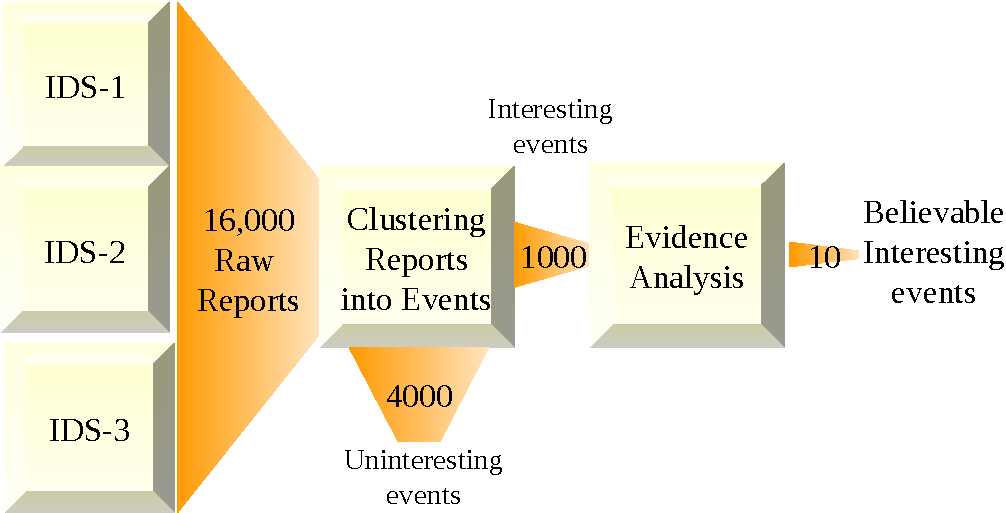
\includegraphics[width=.45\textwidth]{figures/funnel-dup-cropped.pdf} }{%
    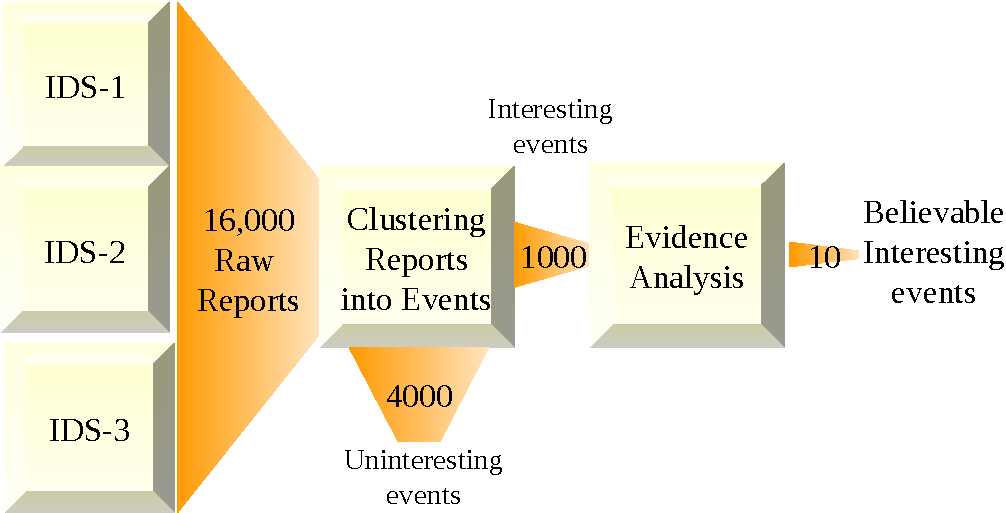
\includegraphics[width=.45\textwidth]{figures/funnel-dup-cropped.pdf}} 
  \centering
  \caption{Scyllarus workload reduction%
% Squash citation here; cited in sentence referencing figure.
%~\anoncite{goldman:09Scyllarus}
.}
  \label{fig:workloadReduction}
\end{figure}



% For example:
% \begin{quotation}
%   Users attending an `ABCs of IDS' event \ldots 
% %at London's City University yesterday 
% said more the 80 per cent of the alerts they received were
% false, with one citing 60 alerts he had received \ldots 
% %about non-existent problems 
% that morning at 0300....
% %The concern is that 
% [A]dopters \ldots
% %of the technology 
% will \ldots %fail to maintain it or 
% simply leave it to gather dust as overworked admins get bombarded with false alarms.~\cite{Register}
% \end{quotation}

% Often the most damning weakness of an IDS is a high false positive rate. 
% In general, with any
% sensor, one must pay in false positives for whatever is gained in
% sensitivity.
%\footnote{Receiver operating characteristic (ROC) 
%curves provide a way of assessing how
%well a particular sensor can provide true detections for a particular
%cost in false positives.  The ROC curve is the curve one gets 
%when plotting $p(\mbox{hit})$ vs $p(\mbox{false positive})$ as 
%the detector's threshold is swept from its most conservative
%to most liberal settings~\cite{MacMillanCreelman:91}.}

% Data reduction, a comprehensive overview, and overcoming false positives and
% false negatives are the goals of \ids fusion.
% Such systems aim to overcome the limitations of existing \idses by assembling 
% a suite of
% sensors.  This can be a very efficient way to overcome the problem
% of false positives, as long as we can find sensors that fail
% relatively independently.  

% A shared framework like ours can also provide protection against
% {\em systematic\/} false positives.  For example, in an early installation of
% \correlator{}, we worked with (an earlier version of) the IDS {\tt
% snort}, which contained rules for detecting IP sweeps.  We found that,
% in sites where \longnav\ were run, this rule was tripped by the normal operation of \nav .
% An automatic update server for \nav\ periodically scanned the network,
% looking for hosts running the \nav\ update client.  
% Such clients listened on
% \navport.\footnote{We are not singling out {\tt snort} for
% criticism.  Our experience has been with {\tt snort}, but
% virtually all network-based \ids es would exhibit this kind of behavior.}

% The ordinary solution to this kind of problem is to edit the \ids\ rule to
% keep it from firing in this circumstance, for example by ignoring IP
% sweeps that hit only \navport .
% This approach is unsatisfactory for two reasons.  First, in sites
% where multiple IDSes are run, this means that we must separately
% update the configuration of each individual IDS.  
% Second, it allows a clever attacker free rein with traffic on this
% port.

% On the other hand, if we have a central repository of this kind of
% information, we get two corresponding advantages:
% First, we have only a single point of update.  Instead of fixing each
% individual sensor, we reconfigure so that all of the reports
% corresponding to this class of false positives will be filtered out.
% Second, we can collect additional information, for example, logs of
% the \nav\ server, that allow us to distinguish between true \nav\
% events, and transmissions from a clever attacker that are disguised as
% \nav\ transmissions.

\draft{Challenges of IDS evaluation}

\paragraph{Related work.}
%% TODO Restore for QR'15
%SecurityFocus has developed the
%Attack Registry and Intelligence Service~\shortcite[ARIS]{ARIS}.
%Its extractor consolidates {\ids} reports from four different
%{\idses} into XML, and presents them in an incident
%console.  However it makes no attempts to fuse the reports, nor weigh
%evidence for and against them.
%
%% TODO Restore full version for QR'15
STAT and MetaSTAT~\cite{vigna01:designing}
use finite-state models to detect and fuse events,
but do not attempt to judge the plausibility of different
events.
%MetaSTAT is a fusion system built on a set of STAT-based
%{\idses}~\cite{vigna01:designing}.  
%STAT is signature-based, and detects events by matching
%against extended finite-state event models.
%MetaSTAT uses
%finite-state models of across-sensor events to consume events
%from lower-level sensors at a higher level,
%but does not attempt to judge the plausibility of different
%events.
EMERALD/eBayes~\cite{raid2001-pac} fusion is the most similar to our systems.
Their sensors are Bayes net-based, and the correlation approach
allows ``upstream'' sensors to adjust the priors on ``downstream''
sensors.
Its fusion is limited to clustering alerts that meet a
similarity criterion; they do not have models of high-level events like
ours (see below).  To the best of our knowledge, they do not
address the difficult issues of acquiring probability parameters for \ids fusion.
The Prelude IDS's Correlator
%% TODO Restore full version for QR'15
% allows users to analyze reports sent to Prelude 
%from compatible IDSes~\cite{PreludeCor} following user-provided
%rules.  Its function
is closest to
our clustering subsystem, but its knowledge resides in stateful 
rules instead of an ontology of attacks~\cite{PreludeCor}. 
%% TODO Restore full version for QR'15
%The Arcsight Enterprise Security Manager~\cite{ArcsightEsm},
%also ties correlated IDS reports to an installation's security goals
%and vulnerability information.


%%% Local Variables: 
%%% mode: latex
%%% TeX-master: "main"
%%% End: 
